\section{Guía de usuario} \label{anex:guia}

La aplicación es muy fácil de usar. Básicamente consiste en un bot de Telegram que controla una \texttt{API} restful que recibe y envía peticiones y respuestas. A través de este bot de Telegram, podremos gestionar el conjunto de módulos de la aplicación para capturar fotos, grabar vídeos, activar el streaming....

Para empezar a utilizar la aplicación, hay que acceder al bot que se ha creado en la aplicación de Telegram. Una vez dentro de la conversación con dicho bot, se puede escribir cualquier letra o número (por ejemplo: `a') o bien el comando \texttt{/start} para activar el menú principal de botones.

\begin{figure}[H]
	\centering
	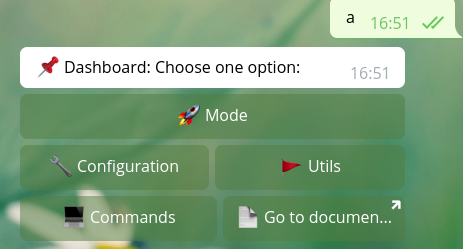
\includegraphics[scale=0.5]{images/59}
	\caption{Menú principal}
\end{figure}

Como se puede observar, hay una interfaz de botones a través de la cual podemos seleccionar las diferentes opciones.

\vspace{-0.4cm}

\begin{itemize}
\item \textbf{Mode:} En esta sección podemos seleccionar el modo de la aplicación. Podemos activar la cámara/vídeo manualmente, activar el sensor de movimiento, el streaming o el filtro de alertas utilizando el detector.

\item \textbf{Configuration}: En esta sección podemos modificar la configuración de la cámara/vídeo, modificando la resolución, rotación, hflip o vflip.

\item \textbf{Utils}: En esta sección podemos visualizar las credenciales del usuario del usuario y bot de Telegram. Esta información puede ser útil, ya que es necesario configurar el bot de Telegram con dichas credenciales para que la aplicación funcione correctamente.

\item \textbf{Commands}: Este botón muestra todos los comandos disponibles para interactuar con la aplicación en lugar de utilizar la interfaz de botones.

\item \textbf{Documentation}: Este botón le redirigirá a la documentación de la aplicación que está disponible en este repositorio.

\end{itemize}

\textbf{Mode}

En esta sección encontrará las siguientes opciones:

\begin{figure}[H]
	\centering
	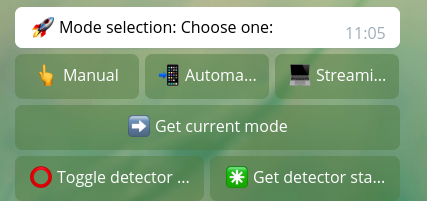
\includegraphics[scale=0.5]{images/60}
	\caption{Menú mode}
\end{figure}

\begin{itemize}

\item \textbf{Manual}: Activa el modo manual. Podrá capturar una foto o grabar un vídeo especificando el número de segundos de grabación. Una vez finalizada esta captura o grabación, se enviará a la conversación.

\begin{figure}[H]
	\centering
	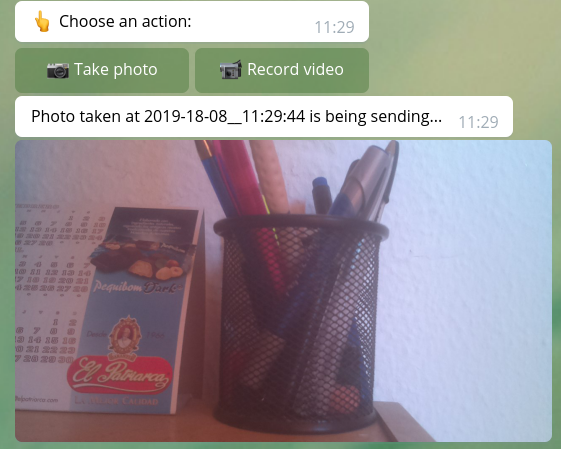
\includegraphics[scale=0.45]{images/61}
	\caption{Captura de una foto en modo manual}
\end{figure}

\begin{figure}[H]
	\centering
	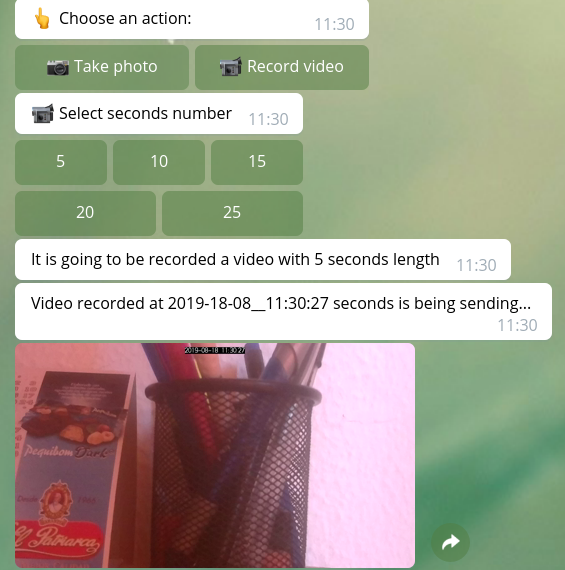
\includegraphics[scale=0.45]{images/62}
	\caption{Grabación de un vídeo en modo manual}
\end{figure}

\item \textbf{Automático}: Activa el modo automático. En este modo se activará el sensor de movimiento y se enviarán alertas cuando se detecte algún tipo de movimiento, y su correspondiente foto o vídeo (según la elección) para poder observar lo que está sucediendo.

\begin{figure}[H]
	\centering
	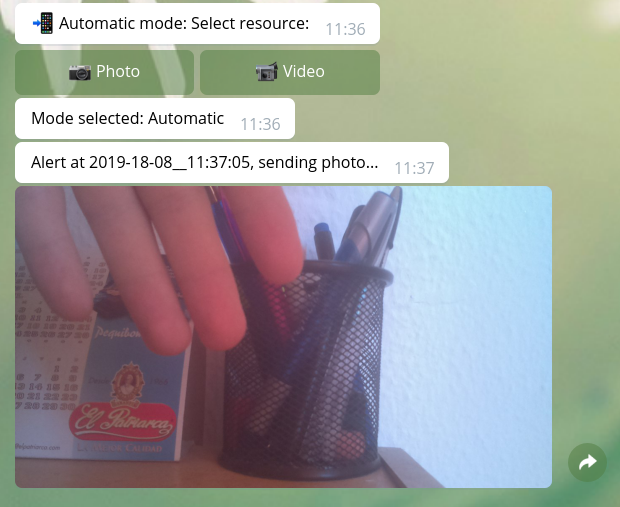
\includegraphics[scale=0.45]{images/63}
	\caption{Imagen y mensaje de alerta tras detectar movimiento}
\end{figure}

\newpage

\item \textbf{Automatic}: Activa el modo streaming. En este modo, podremos observar en tiempo real lo que la cámara está visualizando. Esta retransmisión se realiza de forma responsive, por lo que puede ser visualizada a través del navegador de cualquier dispositivo.

\begin{tabular}{|p{15.5cm}|}
	
	\hline
	
	\textit{ \textbf{Atención:} la emisión no se almacenará, sino que sólo se retransmitirá.}
	\\
	\hline
	
\end{tabular}

\begin{figure}[H]
	\centering
	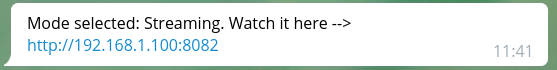
\includegraphics[scale=0.45]{images/64}
	\caption{Enlace a la visualización del streaming}
\end{figure}

\begin{figure}[H]
	\centering
	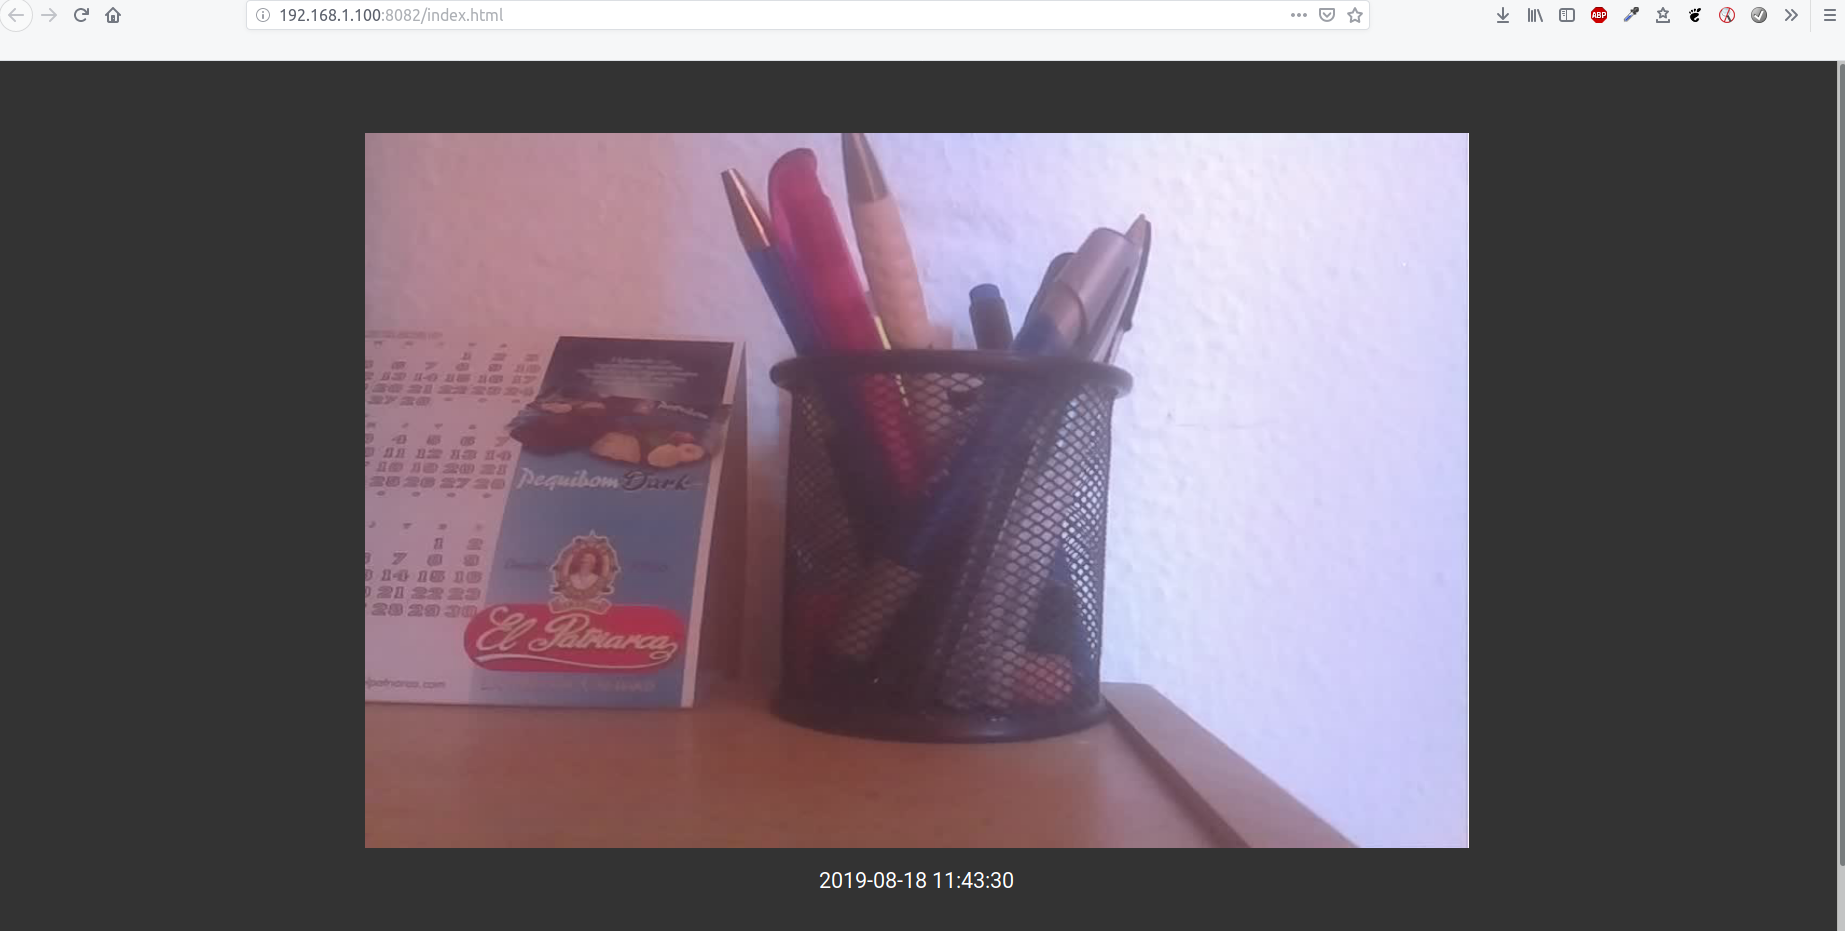
\includegraphics[scale=0.33]{images/65}
	\caption{Visualización del streaming en el navegador}
\end{figure}

\item \textbf{Get current status}: El bot le indicará el modo activo actual

\begin{figure}[H]
	\centering
	
\includegraphics[scale=0.4]{images/66}
	\caption{Modo actual}
\end{figure}


\item \textbf{Toogle detector status}:Activa o desactiva el modo de detector de objetos.

La funcionalidad de este agente es filtrar las imágenes capturadas como alertas, y sólo enviar las alertas en las que se ha detectado a una persona en la foto capturada. Las imágenes catalogadas como `falsos positivos` se enviarán al directorio especificado en el archivo \href{https://github.com/jmv74211/TFM_security_system_PI/blob/master/src/settings.py}{settings.py}.

\vspace{0.3cm}

\begin{tabular}{|p{15.5cm}|}
	
	\hline
	
	\textit{ \textbf{Nota:} 
	    Nota: Es importante saber que sólo tiene que activarse en el caso de una instalación completa y que el proceso del agente detector de objetos está en marcha, por lo que se recomienda configurar una resolución media (1280x720) para la cámara, ya que, por el contrario, el agente tardará demasiado tiempo en procesar la imagen y las alertas tardarán demasiado en ser enviadas a la conversación.}
	\\
	\hline
	
\end{tabular}

 
\begin{figure}[H]
	\centering
	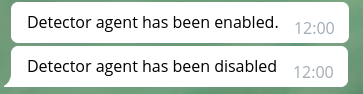
\includegraphics[scale=0.4]{images/67}
	\caption{Encendido y apagado del agente detector de objetos}
\end{figure}

\item \textbf{Get detector status}: El bot le indicará el estado actual del modo detector de objetos.

\begin{figure}[H]
	\centering
	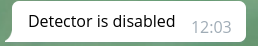
\includegraphics[scale=0.33]{images/68}
	\caption{Estado actual del agente detector de objetos}
\end{figure}


\vspace{0.3cm}

\begin{tabular}{|p{15.5cm}|}
	
	\hline
	
	\textit{ \textbf{Nota:} 
	    Nota: uando se activa un modo, el modo anterior se desactiva automáticamente, es decir, para desactivar un modo, basta con activar otro modo.}
	\\
	\hline
	
\end{tabular}

\end{itemize}

\textbf{Configuration}

En esta sección puede modificar la configuración de la cámara y del vídeo.

\begin{figure}[H]
	\centering
	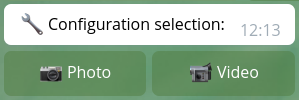
\includegraphics[scale=0.4]{images/69}
	\caption{Menú de configuración}
\end{figure}

\vspace{-0.3cm}

\begin{itemize}

\item \textbf{Photo configuration}

Aquí puede cambiar todos los ajustes de las fotos capturadas tanto en modo manual como en modo automático con fotos.

\begin{figure}[H]
	\centering
	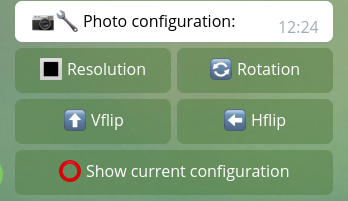
\includegraphics[scale=0.4]{images/70}
	\caption{Configuración de la cámara}
\end{figure}

\begin{itemize}

\item \textbf{Resolution}: Modificar la resolución de la cámara

\begin{figure}[H]
	\centering
	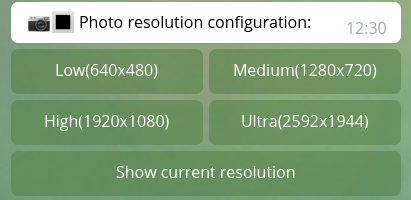
\includegraphics[scale=0.4]{images/71}
	\caption{Configuración de la resolución de la cámara}
\end{figure}

\item \textbf{Rotation}: Modificar la rotación de la cámara

\begin{figure}[H]
	\centering
	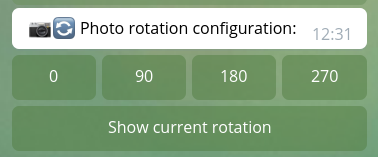
\includegraphics[scale=0.4]{images/72}
	\caption{Configuración de la rotación de la cámara}
\end{figure}

\item \textbf{vflip}: Activar/desactivar el giro vertical de la cámara

\begin{figure}[H]
	\centering
	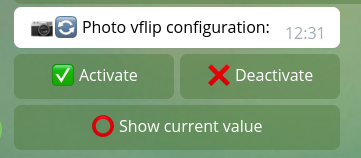
\includegraphics[scale=0.4]{images/73}
	\caption{Configuración del giro vertical de la cámara}
\end{figure}

\newpage

\item \textbf{hflip}: Activar/desactivar el giro horizontal de la cámara

\begin{figure}[H]
	\centering
	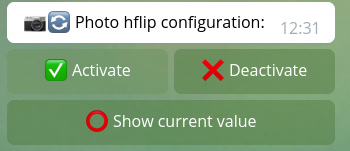
\includegraphics[scale=0.4]{images/74}
	\caption{Configuración del giro horizontal de la cámara}
\end{figure}

\item \textbf{Show current configuration}: Envía un mensaje a la conversación con la configuración actual de la foto.

\begin{figure}[H]
	\centering
	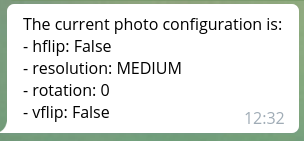
\includegraphics[scale=0.4]{images/75}
	\caption{Configuración actual de la cámara}
\end{figure}

\end{itemize}

\item \textbf{Video configuration}

Aquí puede cambiar todos los ajustes de la grabación de vídeo, tanto en modo manual como automático con vídeo.

\begin{figure}[H]
	\centering
	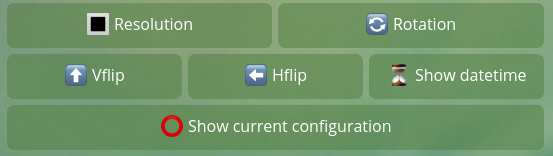
\includegraphics[scale=0.4]{images/76}
	\caption{Menú de configuración para vídeo}
\end{figure}

En la configuración de vídeo, existen las mismas opciones que en la cámara, añadiendo la fecha y hora de visualización, cuyo objetivo es mostrar la fecha y hora de la grabación en la parte superior del vídeo.

\begin{figure}[H]
	\centering
	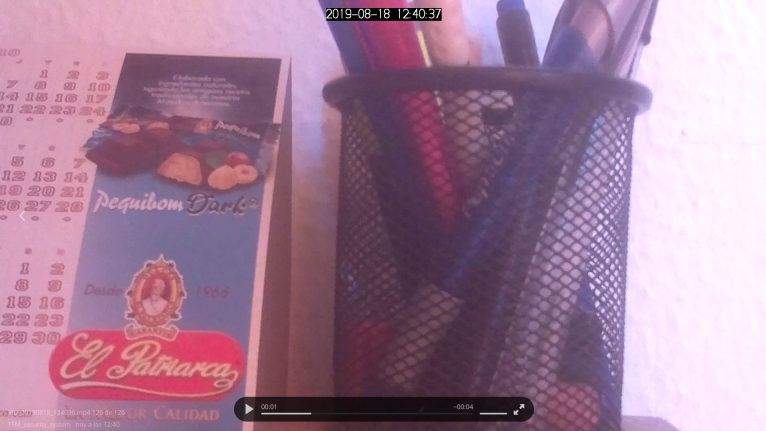
\includegraphics[scale=0.55]{images/77}
	\caption{Vídeo con opción showDateTime activada}
\end{figure}

\begin{figure}[H]
	\centering
	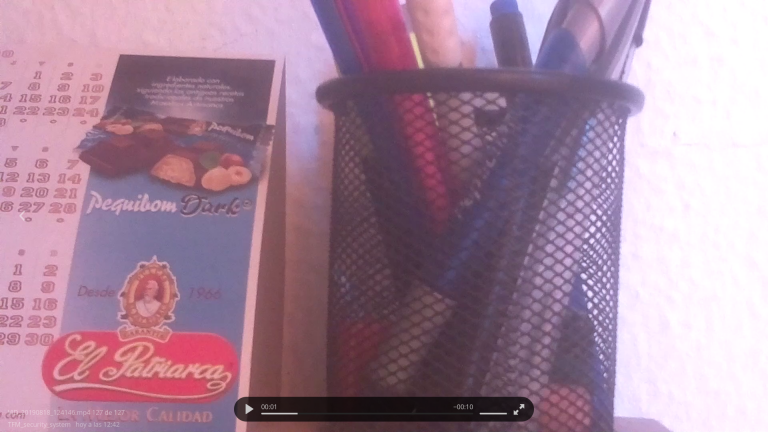
\includegraphics[scale=0.55]{images/78}
	\caption{Vídeo con opción showDateTime desactivada}
\end{figure}

\item \textbf{Utils}

En esta sección podemos visualizar las credenciales del usuario del usuario y bot de Telegram. Esta información puede ser útil, ya que es necesario configurar el bot de Telegram con dichas credenciales para que la aplicación funcione correctamente.

\begin{figure}[H]
	\centering
	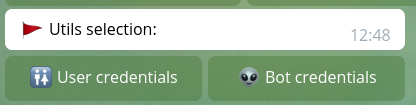
\includegraphics[scale=0.55]{images/79}
	\caption{Menú utils}
\end{figure}

\begin{figure}[H]
	\centering
	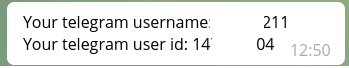
\includegraphics[scale=0.55]{images/80}
	\caption{Credenciales del usuario de Telegram}
\end{figure}

\begin{figure}[H]
	\centering
	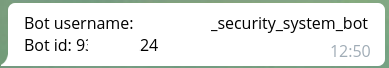
\includegraphics[scale=0.55]{images/81}
	\caption{Credenciales del bot de Telegram}
\end{figure}


\item \textbf{Commands}

Este botón muestra todos los comandos disponibles para interactuar con la aplicación en lugar de utilizar la interfaz de botones.

\begin{figure}[H]
	\centering
	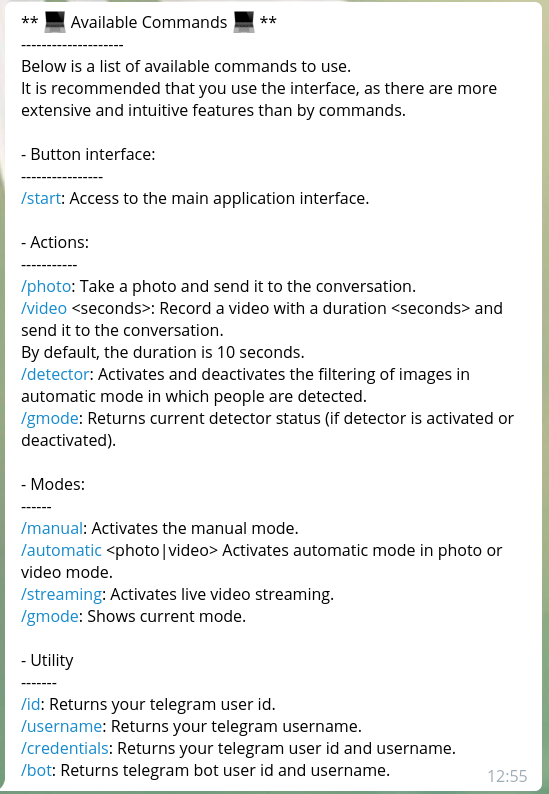
\includegraphics[scale=0.4]{images/82}
	\caption{Lista de comandos disponibles}
\end{figure}

\item \textbf{Documentation}

Este botón le redirigirá a la documentación de la aplicación que está disponible en este repositorio.

\end{itemize}